\documentclass[tikz]{standalone}

\usepackage{tikz}

\def\tikzscale{.7}
\begin{document}


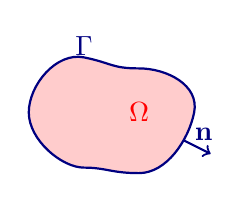
\begin{tikzpicture}[scale=\tikzscale]

  %%\draw[black,fill=blue!20!white]
  %%(0,0) rectangle (5,4);
  
  \begin{scope}[shift={(1,2)}]
    \draw[blue!50!black,thick,fill=red!20!white]
    (0,0) 
    .. controls +( 0.0, 0.5) and +(-0.5, 0.1) .. (1.0, 1.0)
    .. controls +( 0.5,-0.1) and +(-0.5, 0.0) .. (2.0, 0.8)
    .. controls +( 0.5, 0.0) and +( 0.1, 0.5) .. (3.0, 0.0)
    .. controls +(-0.1,-0.5) and +( 0.5, 0.0) .. (2.0,-1.1)
    .. controls +(-0.5, 0.0) and +( 0.4, 0.0) .. (1.0,-1.0)
    .. controls +(-0.4, 0.0) and +( 0.0,-0.5) .. (0.0, 0.0);
  \end{scope}

  %\node[text=blue] at (0.4,0.4) {$\Omega^2$};
  \node[text=red]  at (3.0,2.0) {$\Omega$};
  \node[text=blue!50!black] at (2.0,3.2) {$\Gamma$};
  
  \draw[blue!50!black,thick,->] (3.8,1.5) -- node[near end,above]
  {$\mathbf{n}$} +(0.5,-0.25);

\end{tikzpicture}

\end{document}

%%% Local Variables: 
%%% mode: latex
%%% TeX-master: t
%%% End: 
